\documentclass{article}
\usepackage[utf8]{inputenc}
\usepackage{geometry}
\usepackage{graphicx}
\usepackage{pgfplots}
\usepackage{amsmath}
\usepackage{amssymb}
\usepackage{amsfonts}
\usepackage{mdframed}
\usepackage{amsthm}
\usepackage{tikz}
\usepackage{multicol}

\geometry{a4paper, left=2cm, right=2cm, top=1cm, bottom=2cm}

\pgfplotsset{compat=1.18}
\begin{document}

\begin{minipage}{0.7\textwidth}
    \small \textbf{LABORATORIO DE MECÁNICA VECTORIAL}  \\
    \small {Facultad de Ciencias, Universidad Nacional Autónoma de México} \\
    \small {Profesor: Radamés Ricardo Reynoso Manríquez} \\
    \small {Ayudante: Ana Laura Córdova Lara}\\
    \small {Fecha de entrega: 27 de Febrero de 2024} \\
    \small {Nombre completo: Andrés López González} \\
    \small {Tarea número IV}
\end{minipage}
\hfill
\begin{minipage}{0.12\textwidth}
    
\includegraphics[width=\linewidth]{logo_universidad}
\end{minipage}

\section*{Cuestionario III}

PREGUNTA 1. Defina, en términos del cálculo diferencial e integral, a la velocidad. \\\\
\textit{En este contexto, la velocidad se define generalmente como la tasa de cambio de la posición de un objeto respecto al tiempo $\Vec{r}(t)$, pero hay equivalencias para definirla. Se puede expresar de varias formas dependiendo del enfoque como por ejemplo la ya dicha pero en movimiento undimensional, la velocidad como derivada de primer orden de la posición respecto al tiempo $x(t)$, si la posición de un objeto en un espacio unidimensional se denota como $x(t)$, entonces la velocidad $v(t)$ se define como la derivada de $x(t)$ respecto al tiempo $t$, es decir: $v(t) = \frac{dx(t)}{dt}$; por otro lado está la velocidad como derivadas parciales de cada componente en un espacio tridimensional $\Vec{r}(t)$, si la posición de un objeto en el espacio tridimensional se denota como $\Vec{r}(t)=(x(t),y(t),z(t))$, entonces la velocidad $\Vec{v}(t)$ se define como el vector de derivadas parciales de cada componente respecto al tiempo $\mathbf{v}(t) = \frac{d\mathbf{r}(t)}{dt} = \left(\frac{dx(t)}{dt}, \frac{dy(t)}{dt}, \frac{dz(t)}{dt}\right)$; por otro lado también es posible definirla mediante integrales, la velocidad como la integral del vector aceleración $\Vec{a}(t)$. Si la aceleración se denota como $\Vec{a}(t)$, entonces la velocidad $\Vec{V}(t)$ se obtiene mediante la integración de $\Vec{a}(t)$ con respecto al tiempo $\Vec{v}(t) = \int \Vec{a}(t) \, dt$, recordemos del semestre pasado en física contemporánea que cuando tenemos una función multivariable como lo es $\Vec{a}(t)$ y la queremos integrar respecto al tiempo, obtendremos la velocidad, además la constante de integración en este caso (y debería ser siempre) NO debe pasarse por alto, pues esta representa la velocidad inicial $\Vec{v}_0$.}
\\\\

PREGUNTA 2. ¿Bajo qué criterios o premisas se puede hablar de un movimiento rectilíneo uniforme?\\\\
\textit{El movimiento rectilíneo uniforme (MRU) describe el movimiento de un objeto a lo largo de una trayectoria rectilínea con una velocidad constante en el tiempo. Bajo este tipo de movimiento, el objeto no experimenta cambios en su velocidad ni en su dirección a lo largo del tiempo, lo que lo distingue de otros tipos de movimiento más complejos como lo es su hermano mayor el MRUA. Una característica esencial del MRU es que el objeto se desplaza en línea recta, lo que implica que su trayectoria es una línea recta en el espacio. Esta propiedad simplifica el análisis del movimiento, ya que no se requiere considerar cambios en la dirección del objeto, además que utilizando un cambio de base adecuado este movimiento puede ser descrito con una línea recta muy básica; en un MRU, la velocidad del objeto permanece constante en el tiempo. Esto significa que la magnitud de la velocidad, así como su dirección, no experimentan variaciones a lo largo del movimiento. Esta constancia en la velocidad implica que la distancia recorrida por el objeto en intervalos de tiempo iguales es siempre la misma, lo cual es una implicación directa de que la aceleración del objeto es nula, y esto a su vez nos dice que no existe jerk, snap, crackle, pop, entre otras diferenciales de orden mayor igual a dos en la posición respecto al tiempo. La aceleración se define como el cambio en la velocidad en función del tiempo, y al ser constante la velocidad en un MRU su derivada es cero. Otra derivación de la no existencia de aceleraciones es que en un MRU no hay fuerzas externas actuando sobre el objeto que puedan modificar su trayectoria, en palabras simples, no hay fuerzas de fricción, resistencia del aire u otras fuerzas que puedan alterar su velocidad del objeto.}
\\\\

PREGUNTA 3. ¿Cuál es la diferencia entre un sistema de referencia inercial y un sistema de referencia no inercial? Dé ejemplos de cada uno. \\\\
\textit{Un sistema de referencia inercial es aquel en el que se cumple la primera ley de Newton, en términos simples, un cuerpo en reposo o en movimiento rectilíneo uniforme respecto a este sistema no experimenta fuerzas externas. En un sistema de referencia inercial las leyes del movimiento de Newton se cumplen sin necesidad de introducir fuerzas ficticias o inerciales (como la centrífuga o de Coriolis). Ejemplo de ello podría ser lo siguiente: un avión volando a velocidad constante y altitud constante en el aire desde el punto de vista de un pasajero dentro del avión, si el avión no está acelerando ni girando, se considera que el avión está en un sistema de referencia inercial, en este caso, el pasajero puede soltar un objeto en el interior del avión y observar cómo se mueve con una trayectoria rectilínea y uniforme en relación con el avión, sin la necesidad de invocar fuerzas adicionales más allá de la gravedad y las fuerzas internas normales presentes en el avión; por otro lado, un sistema de referencia no inercial es aquel en el que las leyes del movimiento de Newton no se cumplen directamente, es decir, en el que un cuerpo en reposo o en movimiento rectilíneo uniforme respecto a este sistema experimentaría fuerzas ficticias o inerciales, usando el mismo ejemplo podríamos imaginar que el avión da un giro a la izquierda, esto haría que los pasajeros sientan una fuerza inexistente hacia la derecha descrita como fuerza centrífuga. Estas fuerzas ficticias son necesarias para explicar el movimiento relativo respecto a un sistema en aceleración o rotación. Un ejemplo común de un sistema de referencia no inercial es un automóvil en movimiento, donde los pasajeros sienten una fuerza hacia adelante al acelerar y hacia atrás al frenar, debido a la aceleración o desaceleración del automóvil.}
\\\\

PREGUNTA 4. Explique las aplicaciones de los velocímetros en los dispositivos electrónicos y/o mecánicos. \\\\
\textit{Los velocímetros son dispositivos que según su nombre se intuye que sirven en la medición de la velocidad; en el ámbito de los dispositivos electrónicos, un ejemplo cotidiano es que los velocímetros operan para el monitoreo de la velocidad en vehículos (como los que te toman una foto y te llega la multa a la puerta de tu casa...), automóviles, aviones y trenes. Proporcionan información precisa y en tiempo real sobre la velocidad de desplazamiento, lo que resulta vital para el control y la seguridad durante la conducción. Además, los dispositivos electrónicos de navegación como los sistemas GPS del carro y los teléfonos con funciones de navegación también incorporan velocímetros para estimar en cuánto tiempo llegarás a tu destino (como WAZE que se aprovecha de estos, pues además se sincroniza con las velocidades de los demás conductores que tengan la aplicación activa). En el ámbito mecánico (mecánico en el sentido socialmente consolidado), nos son de ayuda por ejemplo en la industria de fabricación y mecanizado, los velocímetros se utilizan en herramientas de corte, como tornos y fresadoras, para controlar la velocidad de corte; en el sentido físico de la mecánica nos indican la velocidad instantánea de un sistema \textbf{macroscópico} así como molecular dependiendo la complejidad de este, las fotocompuertas empleadas en el laboratorio de momento serán nuestra herramienta estrella, pues nos capturan la velocidad de un objeto bajo condiciones de MRU, aunque también al utilizar dos fotocompuertas podemos obtener la velocidad instantánea en dos puntos del movimiento y acorde a la distancia, velocidad y tiempo que describa el objeto podemos escalar a algo más profundo que la velocidad que es la aceleración en un MRUA.}
\\\\

PREGUNTA 5. Investigue y explique el funcionamiento básico de una fotocompuerta. \\\\
\textit{Las fotocompuertas es un dispositivo que utiliza emisores y receptores de luz para detectar objetos en movimiento. Su funcionamiento básico implica el uso de una señal luminosa de longitud de onda perteneciente a la región infrarroja del espectro electromagnético que se interrumpe cuando un objeto pasa entre el emisor y el receptor (se sugiere, o obliga, que este objeto sea una regleta. Obsérvese en Figure I).}
\begin{figure} [h]
    \centering
    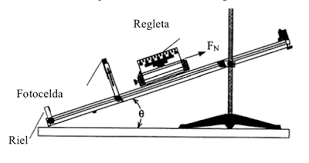
\includegraphics[width=0.45\linewidth]{Regleta.png}
    \caption{Uso práctico de una regleta.}
    \label{fig:enter-label}
\end{figure}\\
\textit{En un movimiento rectilíneo uniforme (MRU), el sensor fotopuerta se coloca en un punto específico de la trayectoria del objeto. Cuando el objeto pasa por este punto, interrumpe el haz de luz que va desde el emisor hasta el receptor, lo que provoca una señal de activación transmitida al smart timer, en términos superficiales es la que da las órdenes y recibe señales de las fotocompuertas, ejemplo de un smart timer muy utilizado en laboratorios es el modelo ME-8930. Ahora, siguiendo al tema, funciona midiendo el tiempo que transcurre entre cada interrupción del haz de luz, es posible determinar el tiempo que el objeto tarda en recorrer la distancia entre dos puntos, para ello necesitamos de dos fotocompuertas, lo que permite calcular su velocidad constante; véase en Figure II cómo es este lindo artefacto.
\newpage
\begin{figure} [h]
    \centering
    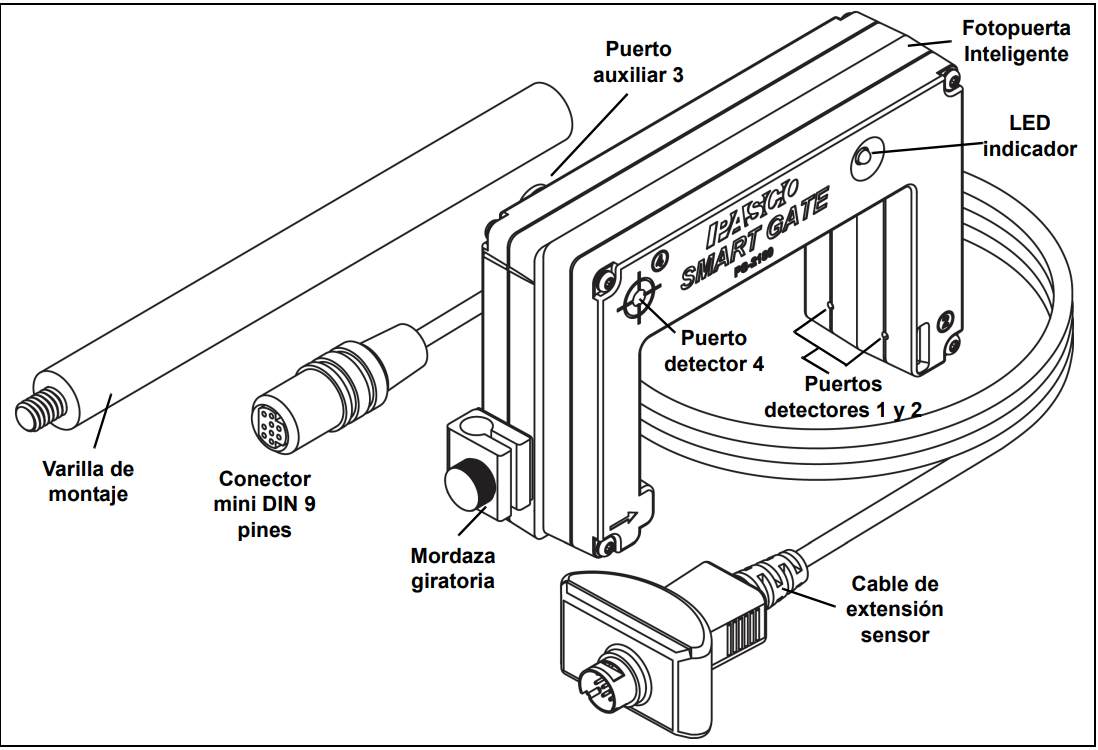
\includegraphics[width=0.75\linewidth]{PASCO.png}
    \caption{Descripción de la fotocompuerta.}
    \label{fig:enter-label}
\end{figure}
Para movimientos circulares o lineales uniformemente acelerados, el funcionamiento es similar, pero con una diferencia crucial en la forma en que se interrumpe el haz de luz. En un MRUA (o su caso particular MCUA), la distancia entre el objeto y el sensor fotopuerta disminuirá con el tiempo, lo que significa que la frecuencia de las interrupciones del haz de luz aumentará con el tiempo. Claro, si la aceleración es negativa es justamente lo contrario, la distancia recorrida respecto al tiempo será cada vez menor y la frecuencia de interrupciones será directamente proporcional a ello.}
\\\\


\end{document}
